

\Chapter{The experiment}{Segregation effect on a granular free-surface flow down a slope.}

\begin{figure}[htp]
\centering
\begin{subfigure}{.5\textwidth}
  \centering
  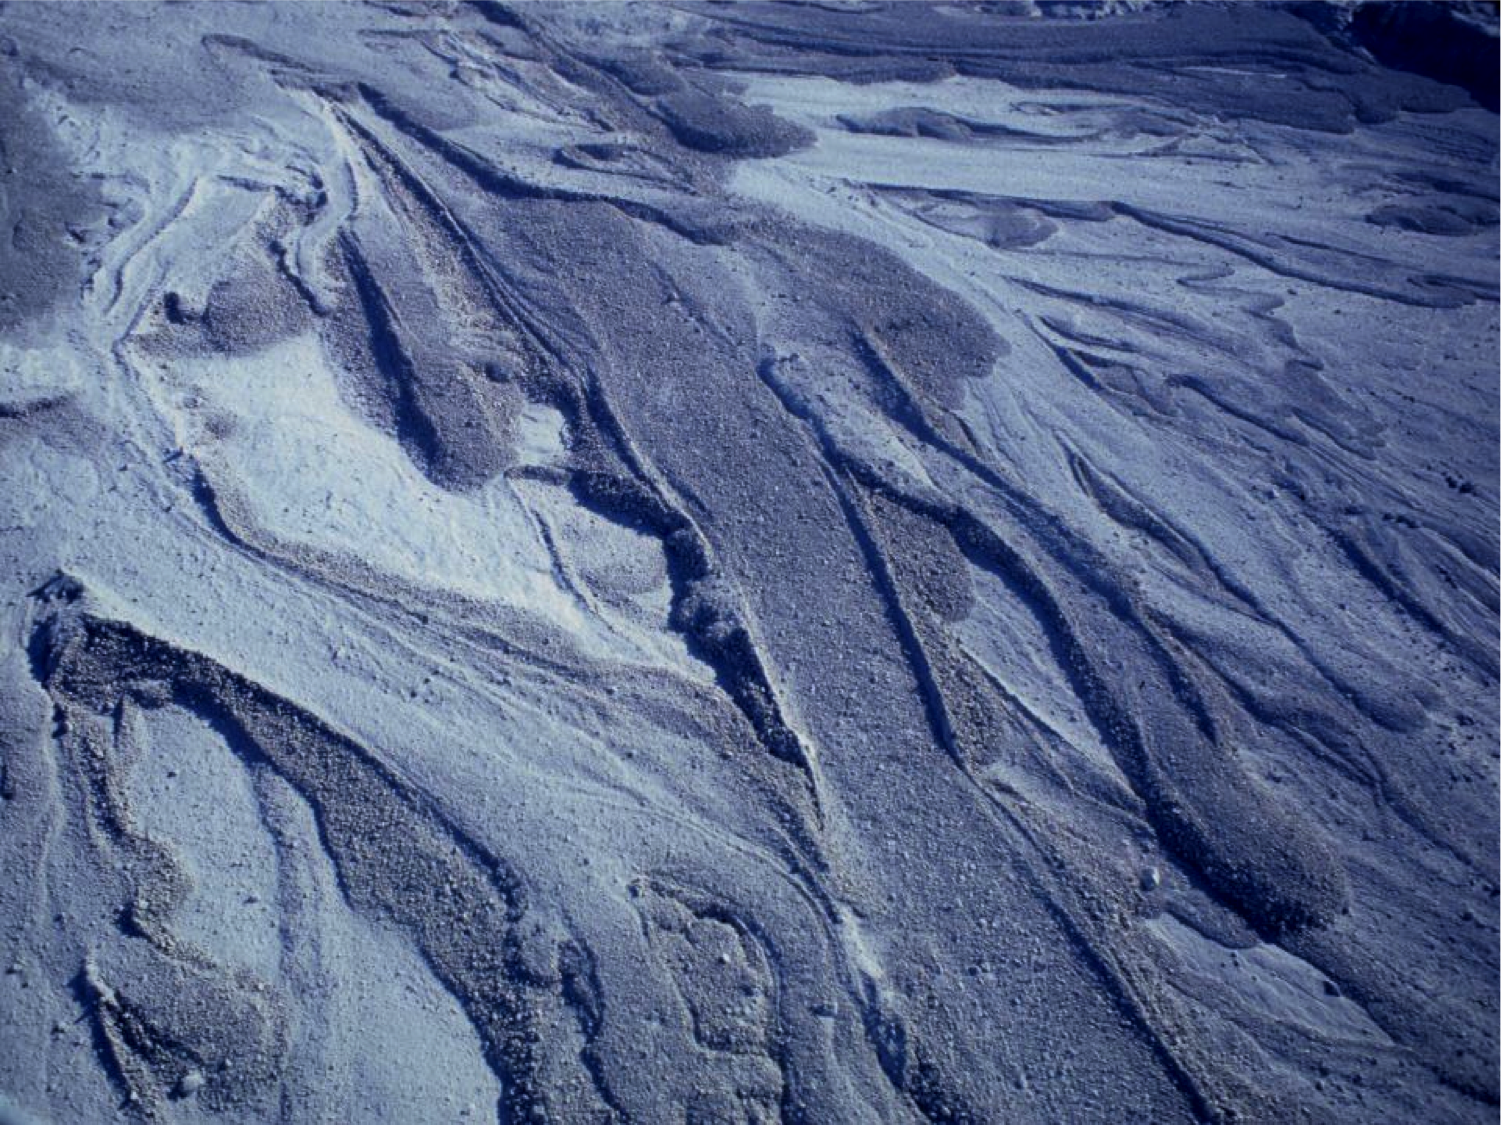
\includegraphics[width=.8\linewidth]{images/st_helen}
  \caption{10 metres wide channels formed by pyroclastic flows after Mount St Helen 1980 eruption.}
  \label{fig:st_helen}
\end{subfigure}%
\begin{subfigure}{.5\textwidth}
  \centering
  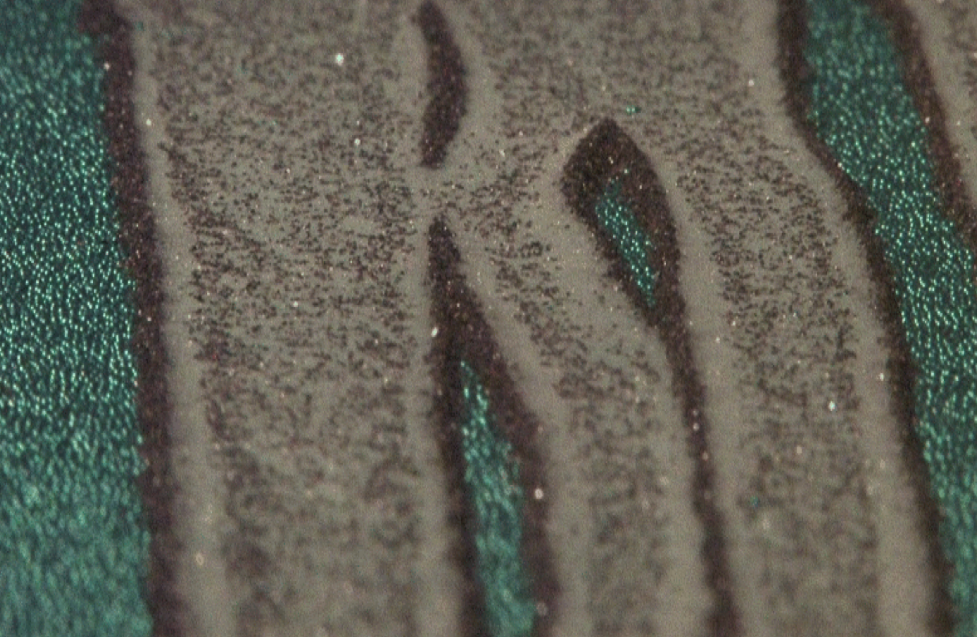
\includegraphics[width=.92\linewidth]{images/small_scale}
  \caption{A small scale experiment housed in the University of Manchester, exhibiting channels approx. 2 cm wide.}
  \label{fig:small_scale}
\end{subfigure}
\caption{Channelisation is a wide-spread phenomenon.}
\label{fig:test}
\end{figure}

Segregation effects in granular avalanches are important as they influence overall flow characteristics. 

In natural granular flows (fig. \ref{fig:st_helen}) and in small scale laboratory experiments (fig. \ref{fig:small_scale}) we observe the formation of lateral levees channelising the flow as it goes down a slope.

Though the remains observed in fig. \ref{fig:st_helen} provide some information on the characteristics of the flow, it is hard to deduce from these observations the process at play before the material came to rest. 
Observing natural granular flows as they occur is impractical, due to unpredictability
and potential dangers. 
Though large scale features can be qualitatively reproduced in the
laboratory, scaling issues can emerge. It is best to develop large scale experiments to simulate natural debris flow characteristics.

\section{The experiment}

\subsection{Setup}

\begin{figure}[htp]
\centering
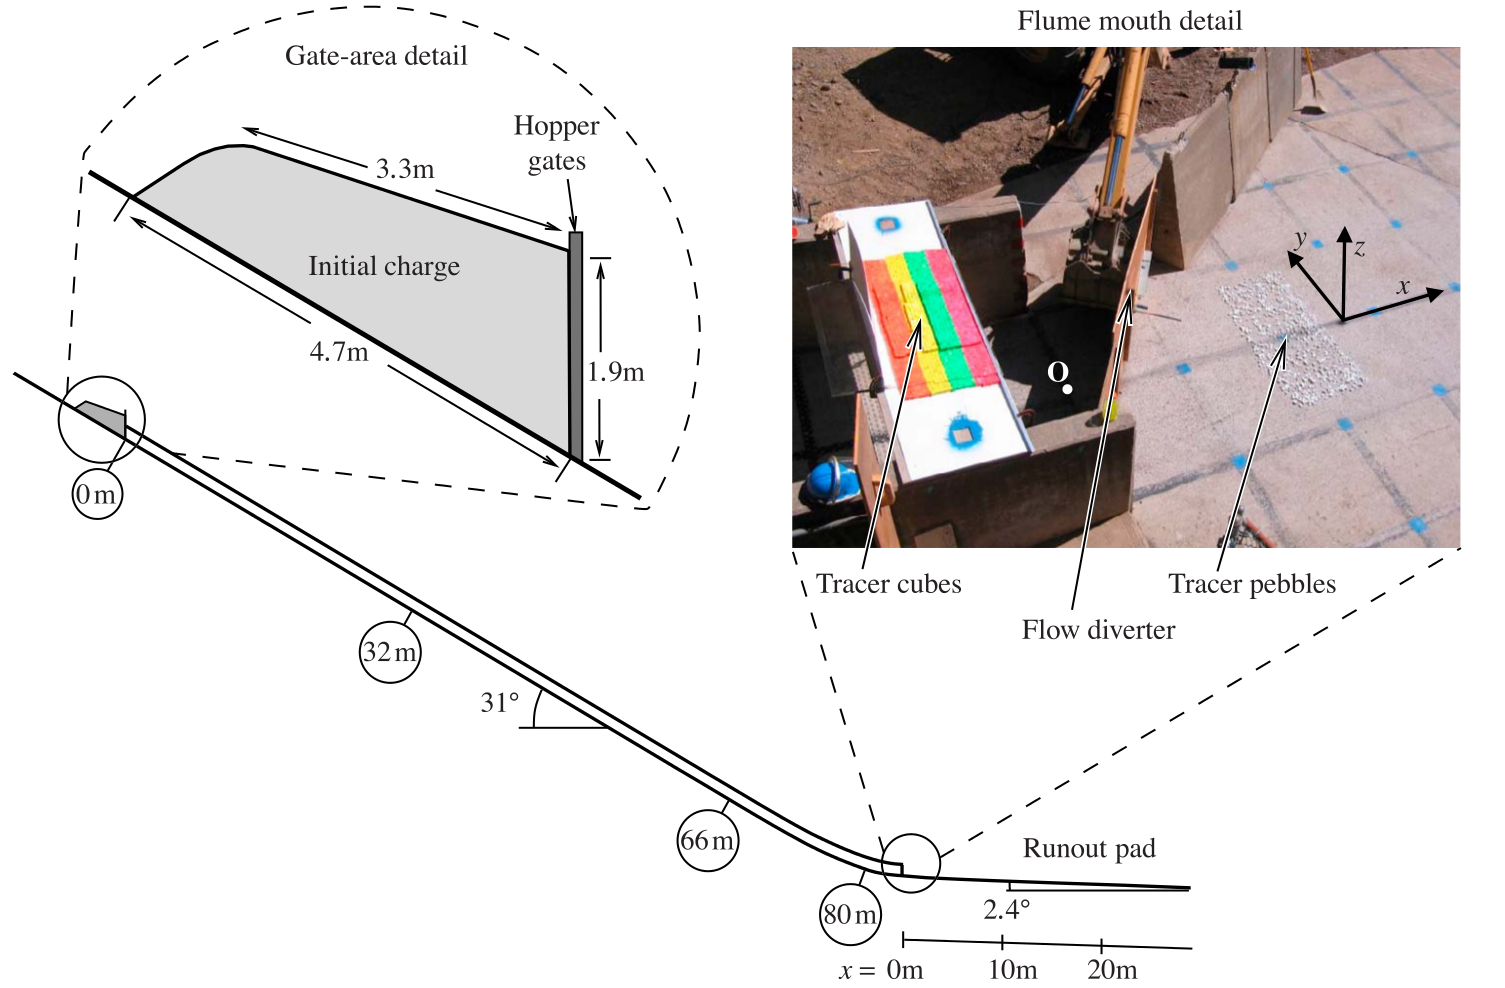
\includegraphics[scale=0.25]{images/whole_flume.png}
\caption{Setup of the large-scale experiment.}
\label{setup}
\end{figure}

A series of two large scale experiments were conducted in August 2011 at the United States Geophysical Survey (USGS) debris-flow flume, near Blue River, Oregon \cite{main}. 

The experimental device consists of a 95 meters long, 2 meters wide inclined channel terminated by a 25 meters long roughly horizontal run-out pad (see fig. \ref{setup}).
A mixture of water saturated sand (0.0625-2 mm) and gravel (2-32 mm) is prepared behind the gates closing the channel entrance.
When the 10 $m^3$ mixture is released, it accelerates and reaches the end of the channel after $\approx 10$ seconds. 
Just after the head of the flow pass the end of the channel, it is truncated and the rest of the flow is diverted (see flume mouth detail in fig. \ref{setup}).
A measurement of the head's surface velocity is performed by ultra-rapid cameras for the first few meters. During the measurement, the head has an approximately constant velocity of $u_F = 2.0$ $m \cdot s^{-1}$. It then slows down; after a few more seconds the material is deposited on the run-out pad.
The rest of the flux is diverted to prevent it to mix with the head on the run-out pad and bury the initial deposit. 

We are interested in studying the last stage of the avalanche, during which the cut head front is going at constant speed on the run-out pad.
In the reference frame travelling at the front speed, we observe that the velocity field is stationary. So in that frame, particle paths coincide with streamlines.

\subsection{General observations}

The surface of the flow is composed of large gravel particles. This is evidence that segregation effects are at play.
Moreover, the formation of lateral levees channelising the flow  is observed. How can we qualitatively account for this observation?

A key feature of the experimental flow, also observed in natural debris flow, is the existence of high sheer rates, both in the direction of the flow, and in the lateral direction.
Sheering in the direction of the flow makes the uppermost layer of particles go faster than the internal layers. When it arrives at the front, it wraps around the head, and the large particles constituting it are buried. 
Because of segregation effects, they are then pushed up. And because of the existence of a high lateral sheer rate, as they go up they will also be pushed to the sides and deposited inside lateral levees.

From this qualitative analysis supported by experimental observations, we deduce that it is the interplay between segregation pushing large particles up, and advection pushing large particles down and to the aisles that is responsible for levee formation and channelisation.
During this internship, we took interest in modelling and explaining in detail this segregation/recirculation effect.

\section{Modelling the experiment}

An option would be to model the experimental flow using fluid equations analogous to the Navier-Stokes equation of fluid mechanics. Prescribing the initial velocity and mass distribution would enable us to deduce the whole evolution of the bulk velocity field.
However, it is not trivial to choose a rheology (ie a granular friction law) adapted to the problem, and at the same time not leading to ill-posedness.
And since measurement of surface velocity and internal shear stress were performed during the experiments, it is natural to prescribe a velocity field agreeing with the measurements, and use it to analyse what is going on inside the flow.
As we said before, during the phase we analyse, the velocity field is stationary in the travelling frame. Starting from this point, every quantity will be expressed in this reference frame. The axis will be chosen accordingly to what is shown in fig. \ref{setup}: the $x$ axis is in the direction of the flow, the $z$ axis is orthogonal to the base, and the $y$ axis is such that the base is orthonormal and positively oriented.

\subsection{Constructing the velocity field}

\begin{figure}[htp]
\centering
\begin{subfigure}{.5\textwidth}
  \centering
  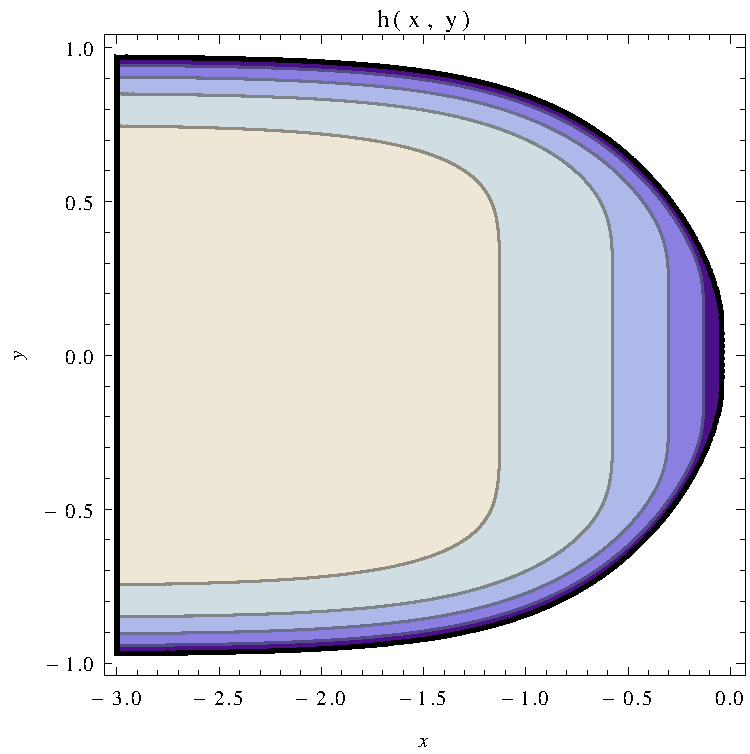
\includegraphics[width=.92\linewidth]{vector/h_contour}
  \caption{Contour plot of the flow head shape $h(x,y)$.}
  \label{fig:h}
\end{subfigure}%
\begin{subfigure}{.5\textwidth}
  \centering
  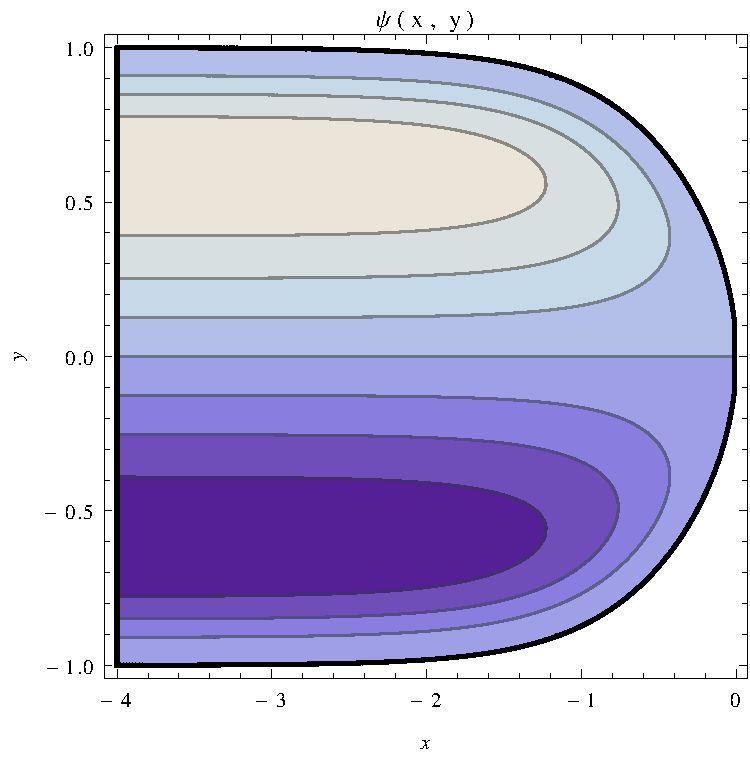
\includegraphics[width=.92\linewidth]{vector/psi_contour}
  \caption{Contour plot of the stream function $\psi(x,y)$.}
  \label{fig:psi}
\end{subfigure}
\caption{}
\label{fig:test2}
\end{figure}

To begin with, we prescribe the shape of the flow surface (fig. \ref{fig:h}). 
There is a general procedure to build a velocity field knowing the flow surface and base, and the \textit{depth-integrated velocity profile}. This quantity is defined as 
\begin{equation}
h(x,y) \bar{u}(x,y) = \int_{z=0}^{z=h} u(x, y, z) dz
\end{equation}

Rather than manipulating the velocity components $u(x,y,z)$, $v(x,y,z)$, $w(x,y,z)$, we will make use of the \textit{depth integrated velocity components} $\bar{u}(x,y)$, $\bar{v}(x,y)$, $\bar{w}(x,y)$. They are defined by
\begin{equation}
h(x,y) \bar{u_i}(x,y) = \int_{z=0}^{z=h} u_i(x, y, z) dz
\end{equation}

Since they only depend on 2 variables instead of 3, they are easier to deal with. In particular, since we assume 3D incompressibility, we have
\begin{equation}
\p{}{x} h \bar u + \p{}{y} h \bar v = 0
\end{equation}

We can thus define $\bar u$ and $\bar v$ by a single scalar field: the stream function $\psi(x,y)$, such that
\begin{align}
\p{\psi}{x} = - h \bar v \\
\p{\psi}{y} = h \bar u
\end{align}

A stream function producing a velocity field in good agreement with the experiments is
\begin{equation}
\psi(x, y) = \frac{H U}{W^2} \left( k y y_0^2 - \frac{k}{2n + 1} \frac{y^{2n+1}}{y_0^{2n-2}} - \frac{1}{2m+1} \frac{y^{2m+1}}{y_0^{2m-2}} + \frac{1}{2n+2m+1} \frac{y^{2n+2m+1}}{y_0^{2n+2m-2}} \right)
\end{equation}
where $H$ is the height of the flow far from the head,  and $W$ and $U$ respectively the typical width and speed of the flow. They are chosen to fit the experimental data.

We have prescribed the depth-integrated velocity field. To compute the full velocity field, we still need a supplementary information, which is provided by the \textit{velocity profile}, containing the $z$ dependency of the velocity components  
It is defined by\footnote{Note that this definition of $f$ implies that $u$ and $v$ have the same $z$ dependency. Though it is not necessarily the case, it has proven a good approximation for the flow we seek to model.}
\begin{equation}
	\begin{pmatrix}
	u(x, y, z)\\
	v(x, y, z)\\
\end{pmatrix}
=
f \left( \frac{z}{h} \right)
\begin{pmatrix}
	\bar u(x, y) \\
	\bar v(x, y) \\
\end{pmatrix}
\end{equation}

Now we have the full velocity profile. We can use it to deduce the evolution of the concentration in small and large particle using the segregation equation we derived in chapter 1:
\begin{equation}
	\p{}{t} \phi + \p{}{x} u \phi + \p{}{y} v \phi + \p{}{z} w \phi - q \p{}{z} \phi( 1 - \phi) = 0
\end{equation}

Solving this equation analytically is difficult. So we would like to solve it numerically, to have an idea of its structure.

\subsection{Numerical simulations}

\begin{figure}[htp]
\begin{center}
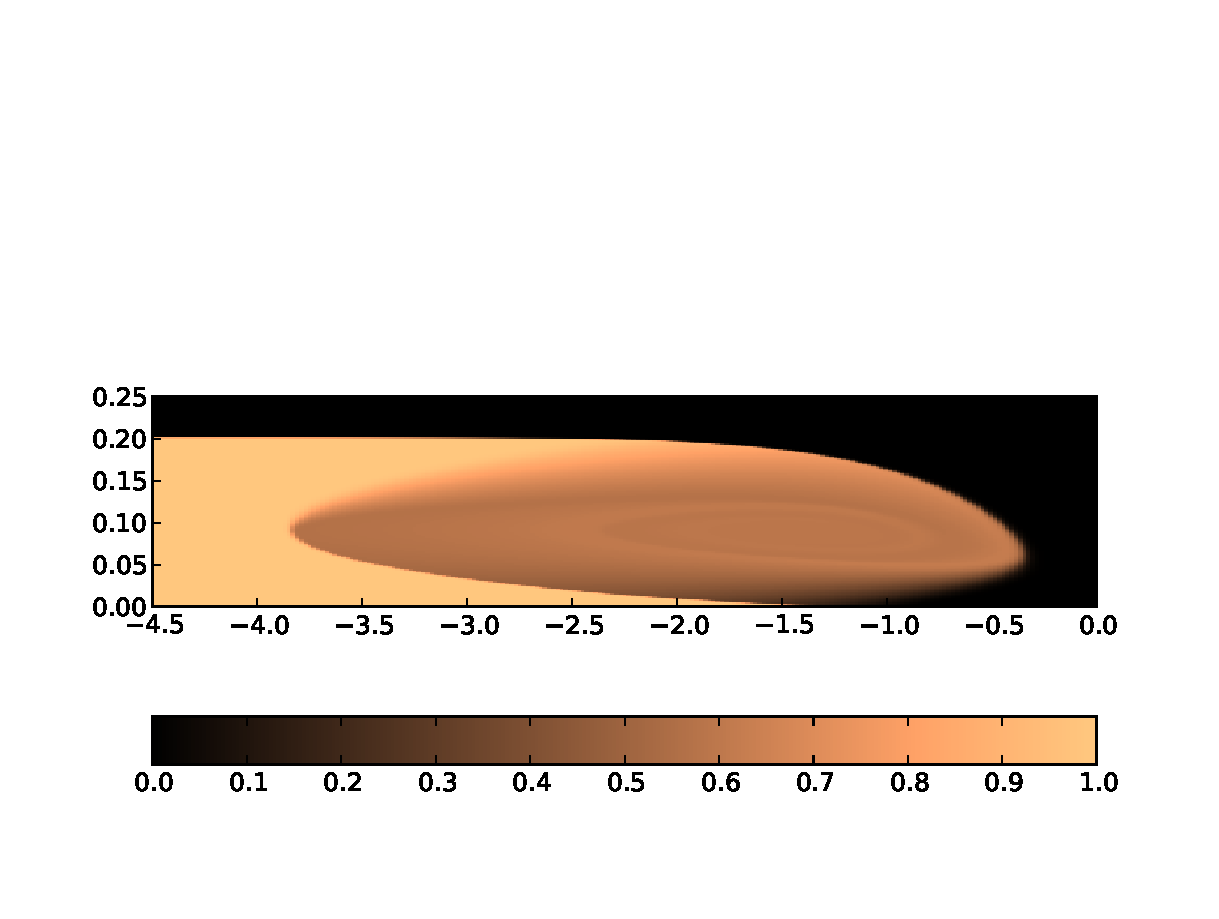
\includegraphics[scale=0.7]{vector/spiral.pdf} 
\end{center}
\caption{Steady-state numerical solution for the 2D problem in the centre plane. \\
Contour plot of the concentration in small particles $\phi$. The darkest, the lowest the concentration is. \\
Quantities are adimensional.}
\label{fig:2D}
\end{figure}

Solving conservation laws numerically is a challenging problem. 
These equations describe quantities that can become discontinuous. For example, a fully segregated granular material is composed of a layer of large particles on top of a layer of small particles. Thus $\phi = 0$ in the upper part of the system, and $\phi = 1$ in the lower part. The two domains are separated by a concentration jump.

Such jumps are difficult to render numerically, as numerical viscosity tends to smooth out discontinuities.

Various approaches can be used to solve conservation laws numerically. We choose to handle the problem using a \textit{finite volume method}. Details about finite volume methods can be found in appendix \ref{app:finite}.

Finite volume methods are exact in the sense that they conserve the solved quantity.
For us, that means that the \textit{numerically computed} total concentration of small particles in the integration domain coincides with the \textit{exact} total concentration, at any time.
This property of conservation is extremely important: it ensures that discontinuities will be accurately calculated by our scheme.\footnote{It can be easily shown (Lax-Wendroff theorem \cite{laxwendroff}) that finite-volume schemes, provided that they converge, will converge to a -perhaps discontinuous- solution of the \textit{exact} conservation law, while non conservative schemes whilst doing as well as finite-volume methods every time the solution is continuous, will cease to be accurate if the solution has discontinuities. Since discontinuities are an essential feature of conservation laws, the conservative property of finite-volume methods is of the highest importance.} 

Far from the head the mixture is fully segregated: it is composed of a layer of large particles ($20 \%$ of the total flow height) on top of a layer of small particles ($80 \%$ of the total height). They are separated by a sharp discontinuity in the concentration $\phi$, called a \textit{shock wave}.
Close to the head, because of the shearing process, the layer of large particles wraps around the layer of smalls. This gives rise to a complex structure, which we would like to explore numerically. 
We set the initial particles to occupy the $0.8$ lowest fraction of the flow height. We then let the system evolve until it reach a steady state. 
Before we simulate the whole $3D$ flow, we will start
with a 2D simulation in the centre plane, ie the plan $y=0$.
  Indeed in this plane, $ \partial v / \partial y = 0$, 
  which means that particles in the centre plane stay in the centre plane. We can rewrite the segregation equation:
\begin{equation}
	\p{}{t} \phi + \p{}{x} u \phi + \p{}{z} w \phi - q \p{}{z} \phi( 1 - \phi) = - v \p{}{y} \phi
\end{equation}
The term $ - v \partial \phi / \partial y$ can be seen as a source term in the 2D problem.
For a brief explanation of how the code I developed during the internship works, see appendix \ref{app:prog}.
The resulting steady-state solution is shown in fig \ref{fig:2D}.

The structure of this solution is higly interesting, and will be analysed in the next chapter.
